\documentclass[12pt]{scrreprt}
\usepackage[utf8]{inputenc}

\usepackage{natbib}
\usepackage{graphicx}
\usepackage{tikz}
\usepackage{pgfplots}
\pgfplotsset{compat=1.12}
\usepackage{textcomp}


\usepackage{amsmath} % Math
\usepackage[parfill]{parskip} % Remove intent on paragraph
\usepackage{caption} % add captions
\usepackage{url} % URLs
\usepackage{hyperref} % Hyperlinks
\usepackage[noabbrev]{cleveref} % Clickalbe hyperlinks



\usepackage[toc, section]{glossaries} % for abbreviation list

\usepackage{mathptmx} % times new roman font
\usepackage{setspace} % line space

\usepackage{tocbibind} % fix for wrong hyperlink for toc, tof and tot

% Remove underfull hbox warnings for bib
\usepackage{etoolbox}
\apptocmd{\thebibliography}{\raggedright}{}{}


\usepackage{enumitem} %list item




% TEMPORARY for writing the report %
% Remember to remove %
%%%%%%%%%%%%%%%%%%%%%%%%%%%%%%%%%%%%%%%%%%%%%%%%%%%%%%%%%%%%%%%%%%%%%%%%%%%%%
\usepackage[inline]{showlabels} % show the label of different figures, tables etc....
\usepackage{xcolor}
% Make pages dark and white text
\pagecolor[rgb]{0.3, 0.3, 0.3}
\color[rgb]{0.9,0.9,0.9}
%%%%%%%%%%%%%%%%%%%%%%%%%%%%%%%%%%%%%%%%%%%%%%%%%%%%%%%%%%%%%%%%%%%%%%%%%%%%%



% Edit the meta.tex file to change title and author names
\newcommand{\mytitle}{Gesture Control with Electromyography}
\newcommand{\myauthor}{Tony Chau}

\title{\mytitle}
\author{\myauthor}
\date{\today}


% Times new romans with 1.15 line-space
\renewcommand{\baselinestretch}{1.15} 

% Over-line over mean variables
\newcommand*\mean[1]{\bar{#1}}


% Add glossarys

%\newglossary[tlg]{abbreviation}{tld}{tdn}{Abbreviations}
\newglossaryentry{IMU}
{
    %type=abbreviation,
    name=IMU,
    description={Inertial Measurement Unit}
} 
 
 
\newglossaryentry{EMG}
{
    %type=abbreviation,
    name=EMG,
    description={Electromyography}
}

\newglossaryentry{MEMS}
{
    %type=abbreviation,
    name=MEMS,
    description={Micro-electromechanical systems}
}

\newglossaryentry{ASL}
{
    %type=abbreviation,
    name=ASL,
    description={American Sign Language}
}

\newglossaryentry{DTW}
{
    %type=abbreviation,
    name=DTW,
    description={Dynmic Time Warping}
}
\glsaddall % to print glossary without references
\makeglossaries



\begin{document}
% The title page
\begin{titlepage}


{\large \today}
\vspace{1.0cm}


\includegraphics[height=1.5cm]{images/ntnu_logo.pdf} 
\vspace{1.0cm}

\begin{center} 
    % Upper part of the page
    TDT4501 - Complex Computer Systems, semester project
    \\
    Fall 2016
    
    ~\\[3.5cm]
    
    \LARGE \textbf{\myauthor}\\[1.5cm]
    
    % Set the title of the Document between two horizontal lines
    \hrule ~\\[0.2cm]
    {\fontsize{25pt}{40pt}\selectfont\mytitle}	% print the title of the document
    \vspace{0.5cm}
    \hrule ~\\[0.2cm]
    
    
    \vspace{1.5cm}
\end{center}




\vfill


\begin{center}
{\large\textbf{Supervisor:}}
\\
Stefano Nichele
\end{center}
\vspace{0.5cm} 




%\vspace{1.0cm} 

%\large{Norwegian University of Science and Technology
%\\[0.2cm]
%Faculty of Information Technology, Mathematics and Electrical Engineering
%\\[0.2cm]
%Department of Computer and Information Science} 

\end{titlepage}

\vspace*{\fill}
{\centering\huge\bfseries Abstract \par}
The Myo armband is a wearable gesture and motion control device that uses a set of electromyographic sensors that sense electrical activity, combined with a gyroscope, accelerometer and magnetometer, to recognize gestures. This report will present a development of a prototype-level system that use the Myo armband to detect and translate simple hand gestures to something coherent.

About 70 million deaf people use sign language as their first language or mother tongue, but the lack of a common language between deaf and hearing individuals makes communication difficult. This report aims to explore the potential of utilizing electromyography and Inertial Measurement Units to help communication between deaf and hearing individuals.
\vspace*{\fill}
\thispagestyle{empty}

\clearpage
\pagenumbering{Roman}
\setcounter{page}{1}


\tableofcontents
\clearpage

\listoffigures
\clearpage

\listoftables
\clearpage

\pagenumbering{arabic}
\setcounter{page}{1}

% Main matter - edit corresponding file under content/ to change
\chapter{Introduction}
\label{chap:introduction}

\section{Motivation}
\label{sec:motivation}
People tend to move their hands when they talk, they make gestures.  Gesturing is a known phenomenon, found across cultures, ages, and work. Gestures are even found in individuals that are blind from birth \cite{goldin1999role}. Body movement is a powerful medium for non-verbal interaction \cite{caramiaux2015understanding}. If computers were trained to recognize gestures on top of the traditional User Interface (UI) elements, like text input and speech, we could expand for better expressions and new control alternatives. Speech is a very natural way of communicating, but sound may be inappropriate in certain circumstances that require silence, such as police infiltration operations, or even impossible for the case of deaf people \cite{paudyal2016sceptre}. 

Sign language is a form for human communication based on visual perception. According to World Federation of the Deaf, there are about 70 million deaf people who use sign language as their first language or mother tongue \cite{wfdeaf:sign_language}. Deaf and hard-hearing individuals, who learn the sign language from an early age have to learn both the signed and non-signed varieties that co-exist in the society \cite{bidoli2008english}. The majority of our society do not have a common sign language, and do not have the ability to understand well developed sign languages, such as the American Sign Language (ASL). Communication difficulties between deaf people and hearing people is a consequence of lack of a common language.

An utility device made for translating signed language, can be beneficial for user-to-user communication. Take a scenario where at least one of the involved in the communication wish to communicate using a gesture based form of communication, while the other involved do not have the ability to understand this form of communication. A device capable of this is not only useful for sign language translation, but in every context where gesture based communication is required, such as military communication or other circumstances where sound could be dangerous.


\section{Problem description}
\label{sec:problem_description}
The Myo armband is an off-the-shelf gesture recognition device that uses a set of electromyographic sensors that sense electrical activity in the forearm, combined with a gyroscope, accelerometer and magnetometer to recognize gestures. It can also give haptic feedback vibrations.

\begin{sloppypar}
Electromyography (EMG) is an electrodiagnostic medicine technique for evaluating and recording the electrical activity produced by skeletal muscles. An electromyograph detects the electrical potential generated by muscle cells.
\end{sloppypar}

The goal of this report is not to describe the development of a product, but rather explore capabilities and applications of using electromyography and orientation in gesture control. This report will deal with using the Myo armband to detect muscle gestures with the goal of helping communication of people that rely on arm/hand signals, such as orchestra director, traffic policeman, football referee hand signals, deaf people, military signals, construction site, and hand signals.

\section{Project Scope and Outline}
\label{sec:project_scop_and_outline}
This report will describe an implemented system to recognize gestures using the Myo armband. The system will be used to explore capabilities and applications of utilizing electromyography and IMU, and will not focus on optimizations regarding speed or user experience. 

We will first take a look on related work in \cref{chap:background}. Then move on to a detailed description of the technology provided by the Myo Armband in \cref{chap:myo} and \ref{chap:theory}. In \cref{chap:methodology} we will cover the description of the implemented system. Technical details and mathematical models will also be provided in this chapter. Methods for testing and the received result is propsed in \cref{chap:results}. The last part of the report, \cref{chap:discussion} and \ref{chap:conclusion}, will provide an analysis of the system and the results, and discusses any potential improvements. 
\chapter{Background}
In this chapter we will take a look at other relevant work where the Myo armband or in general EMG have been used for similar or related applications.

\section{EMG-based Controlled Robot}
Various interface systems and prosthetics have been developed to support handicapped people with limit manipulation capability of the upper limb due to traffic accident, cerebral apoplexy, or other afflictions. Many prosthetic arms have been developed for amputees since the 1970’s, and in \cite{fukuda1998emg}, the concept of an EMG-based human-robot interface as rehabilitation aids is proposed. In \cite{artemiadis2010emg}, a methodology for controlling an anthropomorphic robot arm using nine surface EMG electrodes to record the muscular activities is proposed. A control interface is proposed, according to which, the user performs motions with his/her upper limb. The recorded electromyographic activity of the muscles can be transformed into kinematic variables that are used to control an anthropomorphic robot arm.

In \cite{cnet:myoarm}, a project where amputee Johnny Matheny lost his arm to cancer in 2008. At the Johns Hopkins Applied Physics Laboratory, Matheny worked with a prosthetic arm attached directly to his skeleton, this prosthetic arm is controlled by the use of two Myo armbands on his upper arm that detect the electrical activity of his muscles.
\section{Gesture Recognition}
The study of human-computer interaction has developed to put a significant amount of effort in on user-friendly interfaces employing voice, vision, gesture, and other innovative I/O channels. One of the most challenging approaches in this research field is to link neural signals with computers by exploiting the electrical nature of the human nervous system. The development of an EMG-based interface for hand gesture recognition is presented in \cite{kim2008emg}, where an EMG-sensor is positioned on the inside of the forearm to recognize control signs in the gestures.

Gesture-based control is one of the major application for hand gesture recognition technologies. Another major application is sign language recognition. Sign Language recognition aim to help the deaf communicate with the hearing society conveniently. This paper \cite{zhang2011framework} presents a framework for hand gesture recognition based on the information of a three-axis accelerometer and multichannel EMG sensors.

\section{SCEPTRE}
This report is mainly based on a project called SCEPTRE by some researchers from Arizona State University \cite{paudyal2016sceptre}. The primary goal of SCEPTRE is to match gestures.

The system SCEPTRE is comprised of an Android smartphone or a Bluetooth enabled computer and one to two Myo devices. The goal is to develop a system using two Myo devices to decipher American Sign Language (ASL) gestures, and display the meaning on a smartphone or computer. SCEPTRE utilizes the data from the accelerator, magnetometer, and EMG-sensors. The project is an attempt to develop a system toward a system which is ubiquitous, non-invasive, works in real-time, and can be trained interactively by the user. 

The system is envisioned to be used in two primary use cases:
\begin{itemize}
    \item User-to-User interaction
    \item User-to-Computer interaction
\end{itemize}

20 ASL sign with training instances for each gesture were chosen to prototype test the system. It is also possible for the user to train the system with additional signs, either in "guided mode" or "ASL mode". In guided mode the system compare the new gesture data with the existing data collection to ensure there are no clashes, meaning too much overlapping data, the ASL mode does not make this guarantee.

Dynamic Time Warping (DTW) is used to compare accelerometer and orientation data. DTW is a technique to find an optimal alignment between two given (time-dependent) sequences. For the EMG-data an energy based comparison was used. By using a combination of data from the accelerometer, magnetometer and EMG-sensors the system was able to archive an accuracy of 97\%. 
\section{Alternative Gesture Control Methods}
\sloppy
The ability of tracking position and movement for gesture recognition can be archived by various approaches. The Myo armband uses accelerometer, gyroscope, and magnetometer to keep track of the orientation, and EMG-sensors to measure electric activity of the muscle. Other tool such as Kinect and Leap Motion is based on a more visual approach. 

\subsection{Gesture Gloves}
Hand gestures is movements of the arms and fingers, and one possible approach to track movement of the arms and fingers is to place sensors directly on the fingers, for example in the form of a glove. Two University of Washington undergraduates have won a \$10,000 Lemelson-MIT Student Prize for gloves that can translate sign language into text or speech \cite{uw:SignAloud}. Another example is the out-of-the-self gesture glove from Maestro Gesture Glove \cite{maestroglove}.

\subsection{Image-based Gesture Control}
Leap Motion \cite{leap_motion} and Kinect \cite{kinect} are two commonly used sensors for tracking motions by utilizing technology such as infrared cameras, infrared LEDs, RGB camera, and depth sensor. Unlike the other mentioned devices, Leap Motion and Kinect observe the movements, instead of touching the user. Leap Motion and Kinect utilize different technologies, thus have different advantages and disadvantages, but conceptually, they work in the same manner. There are some different ASL related work based on both Leap Motion \cite{potter2013leap,chuan2014american} and Kinect \cite{zafrulla2011american,lang2012sign,chai2013sign}, but also work that tries to utilize the advantage of both by combining the sensors \cite{marin2014hand}.
\chapter{The Myo Armband}
\label{chap:myo}
This report is based on the use of the Myo armband, and this chapter will cover a brief description of the Myo device, such as hardware specification and software functionality. The Myo armband, developed by Thalmic Labs, is a wearable gesture and motion control device that uses a set of electromyographic (EMG) sensors that sense electrical activity, combined with an Inertial Measurement Unit (IMU) including gyroscope, accelerometer and magnetometer, to recognize gestures \cite{myo}.

\begin{figure}[ht]
    \centering
    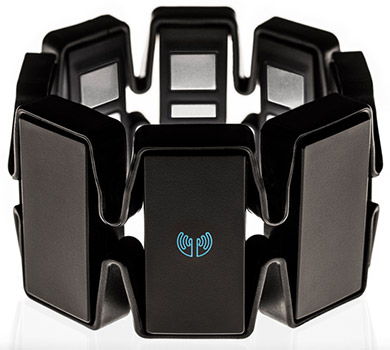
\includegraphics[height=5cm]{images/myoarmband.jpg}
    \captionsource{\url{https://s3.amazonaws.com/wordpressprod/blog/wp-content/uploads/2014/06/front-view.jpg}}
    \caption[The Myo Armband]{The Myo Armband}
    \label{fig:myoarmband}
\end{figure}


\section{Hardware}
The Myo armband consist of eight EMG sensors and nine-axis IMU containing gyroscope, accelerometer and magnetometer. The hardware specification is shown in \cref{table:myo_hardware}.

\begin{table}[ht!]
\centering
    \begin{tabular}{ | l | p{8cm} |}
        \hline
        \textbf{Sensors} & EMG sensor,\newline Gyroscope,\newline Accelerometer, \newline Magnetometer\\ \hline
        
        \textbf{Processor} & ARM Cortex M4 Processor  \\ \hline
        
        \textbf{Feedback} & Dual Indicator LEDs,\newline Short, Medium, Long Vibrations  \\ \hline
    \end{tabular}
    \caption[The Myo Hardware]{List of The Myo Hardware specifications}
    \label{table:myo_hardware}
\end{table}

\section{The Myo SDK}
\label{sec:myoSDK}
Thalmic Labs provides a SDK that allows developers to obtain access to the data from the Myo device. Since the Windows SDK was used, every statements in this report will be based on the Windows SDK. The library at the core of the Myo SDK allows applications to interact with the Myo armband. All functionality in libmyo is exposed through a plain C API. Typically, applications do not interact with the libmyo C API directly. Instead they use a language binding corresponding to the programming language used by the application \cite{myoSDK}.

\Cref{fig:myoSDKstack} illustrates the Myo development stack from an application using the SDK down to a physical Myo device

\begin{figure}[ht]
    \centering
    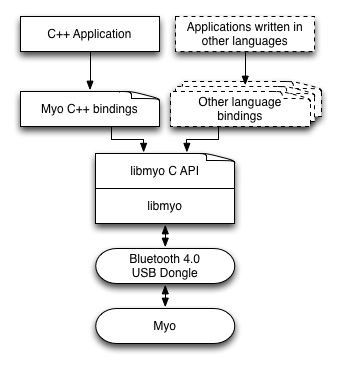
\includegraphics[height=10cm]{images/myo-sdk-stack.png}
    \captionsource{\url{https://developer.thalmic.com/docs/api_reference/platform/the-sdk.html}}
    \caption[The Myo SDK stack]{The Myo SDK stack: Myo development stack from an application using the SDK down to a physical Myo device}
    \label{fig:myoSDKstack}
\end{figure}

The Myo armband provide applications with two type of data: Spatial data and gestural data.

\subsection{Spatial Data (IMU)}
Spatial data represents the location of the armband, and informs the applications about orientation and movements. This data is provided by the IMU. The Myo armband output three different data from the IMU: 
\begin{itemize}
  \item raw Accelerometer data
  \item raw Gyroscope data
  \item Orientation data
\end{itemize}
All which has a frame rate of 50 hz. Accelerometer data and gyroscope data is represented as 3D-vectors, with the unit g-force (accelerometer) and deg/s (gyroscope), while the orientation data from the magnetometer is represented as quaternions.

\subsection{Gestural Data (EMG sensor)}
\label{subsec:myoEmgSensor}
Gestural data provide applications with information of less orientation depended movements, such as hand gestures. This data is provided by the EMG sensors. The Myo armband have eight EMG sensors, which outputs raw EMG data of 8-bit with a frame rate of 200 Hz \footnote{\url{http://developerblog.myo.com/raw-uncut-drops-today/}}. The MyoSDK documentation \cite{myoSDK} doesn't exactly provide information about the measurement unit, but the values are converted into a 8-bit value ranging from -128 to 128.
\chapter{Theory}
\label{chap:theory}

\section{Electomyography (EMG)}
Electromyography (EMG) is an electrodiagnostic medicine technique to measure muscle response or electrical activity produced by skeletal muscles \cite{wiki:Electromyography}. The nerves control the muscles by electrical signal called impulse, these impulses can be measured and analyzed \cite{WebMD:Electromyogram}. There are different method to measure those signals, but this report will only cover the use surface EMG. Surface EMG is a technique where electrodes are places on the skin overlying a muscle to detect nerve impulses. 

EMG can be used to sense isometric muscular activity which does not translate into movement. This make it possible to detect motionless gestures. One of the main difficulties in analyzing the EMG signal, is the noisy characteristics. Compared to other bio-signals, EMG contains complicated types of noise that are caused by, for example, inherent equipment noise, electromagnetic radiation, motion artifacts, and the interaction of different tissues. Hence, pre-processing is needed to filter out the unwanted noises in EMG \cite{kim2008emg}. Because surface EMG does not get direct measurement of the motor unit activation and many factors can influence the signal, these relations are frequently misinterpreted. Although surface EMG is a useful measure of muscle activation, there are limits to the information that can be extracted from the signals \cite{farina2004extraction}.
\section{Inertial Measurement Unit (IMU)}
An inertial measurement unit (IMU) is an electronic device that measures linear and angular motion, usually with the combination of accelerometers and gyroscopes, but sometimes also with magnetometers. As described in \cref{chap:myo}, the Myo armband provide data from accelerometer, gyroscope and magnetometer. These are three sensors useful to determine position and orientation, but they measure different things.

\subsection{Gyroscope}
The gyroscope is used to measure or maintain the angular position. It consist of a disc (the rotor) that spins about an axis. Based on the principle of conservation of angular momentum, a spinning rotor will maintain it's orientation, thus the axis will be unaffected by tilts or rotations \cite{gyroscope_demonstration_project}. We can separate gyroscopes into three basic types:

\begin{itemize}
    \item Rotary (classical) Gyroscopes
    \item Vibrating Structure Gyroscopes
    \item Optical Gyroscopes
\end{itemize}

The gyroscope measure the angular velocity of the rotor. Since vibrating structure gyroscopes with MEMS technology are widely used in smart-phones and other electronic devices, we will take a closer look on vibrating structure gyroscopes \cite{wiki:Vibrating_structure_gyroscope}. To better understand vibrating structure gyroscopes we need a basic understanding of the Coriolis effect. Every point on a rotating system will have the same angular velocity, but in order to travel a straight line towards or away from the axis of rotation, the traveling object have to either increase or decrease the linear velocity in order to maintain the relative angular position. The acceleration required to maintain the relative angular position is the Coriolis acceleration, an example is shown in \cref{fig:coriolis_acceleration} \cite{vibrating_structure_gyroscope}. Vibrating object tends to continue vibrating in the same plane even if its support rotates. The Coriolis effect causes the object to apply a force on its support, and by measuring this force, the angular velocity can be determined \cite{wiki:Vibrating_structure_gyroscope}.

\begin{figure}[ht]
    \centering
    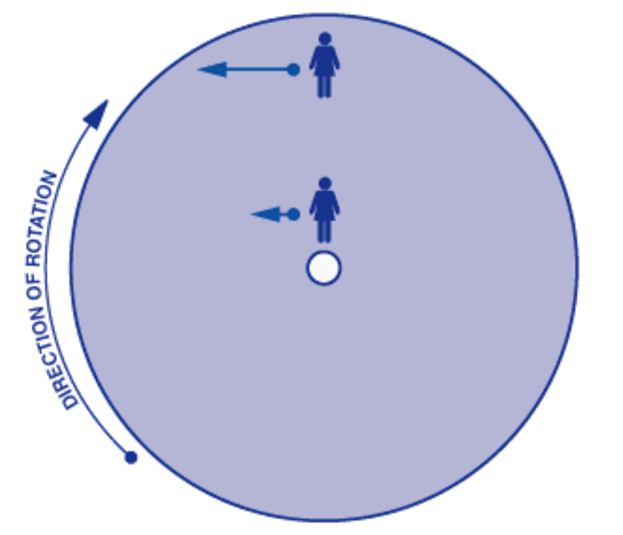
\includegraphics[height=5cm]{images/coriolis_acceleration.jpg}
    \captionsource{\url{http://www.analog.com/en/analog-dialogue/articles/imems-angular-rate-sensing-gyroscope.html}}
    \caption[Coriolis Acceleration Example]{A person trying to move northward toward the outer edge of a rotating platform. The linear velocity (Blue linear arrows) has to increase in order to maintain a northbound course. The acceleration is the Coriolis acceleration.}
    \label{fig:coriolis_acceleration}
\end{figure}


\subsection{Accelerometer}
An accelerometer is an electromechanical device to measure proper acceleration. Proper acceleration should not be confused with coordinate acceleration (rate of change of velocity). The measurement unit is given by g-forces ($g \approx 9.81m/s^{2}$), and by contrast to measuring coordinate acceleration, accelerometers in free fall will measure zero. 

There are many type of accelerometers, but to understand how the accelerometer work, we can use a simple model. Have in mind that this model is not exactly how a MEMS sensor work, but it explains the basic concept of accelerometers. To make this model simple, we will use a representation as shown in \cref{fig:accelerometer_model}. Imagine a ball inside a cube, when gravity pulls the ball down, it will hit at least one of the walls. The wall will according to Newton's third law have a force against the ball. This force is the measurement the accelerometer returns. This value can be represented by a vector \cite{IMU_guide}.

\begin{figure}[ht]
    \centering
    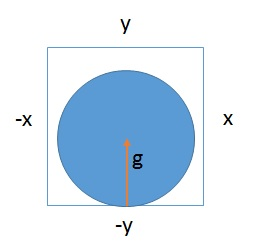
\includegraphics[height=5cm]{images/accelerometer.jpg}
    \caption[Accelerometer model]{2D representation model of a simple concept of an accelerometer. A ball is pushed down by gravity, and the accelerometer measure 1g at the -y wall.}
    \label{fig:accelerometer_model}
\end{figure}

\subsection{Magnetometer}
Orientation of a static or slow-moving rigid body can be determined from the measured gravity and local magnetic field vectors \cite{yun2008simplified}. Magnetometer is a device that measure magnetic fields, either the magnetization of magnetic materials, or the strength and the direction of the magnetic field at a point in space \cite{wiki:Magnetometer}. By measuring earth's magnetic field, a magnetometer can be used to detect the orientation. The magnetometer from the Myo armband returns the orientation as unit quaternion \cite{myoSDK}. Quaternions provide a mathematical notation for representing orientation and rotation in the three dimensional space. Quaternions is described in more detail in \cref{sec:quaternion}.
 

\section{Orientation Quaternions}
\label{sec:quaternion}
Euler Angles is one way to represent orientation, and it is based on that any orientation can be archived by rotations about the axes of a coordinate system. Compared to quaternions, Euler angles is simple and intuitive, but there are some ambiguities, one of those is the gimbal lock. In simple terms, gimbal lock is when two of the axis line up, and cause the rotating object to lose a degree of freedom. Quaternions introduce another approach to represent orientation that do not suffer from the gimbal lock, but is in return less intuitive and mathematically more complicated. This section will give a brief introduction to orientation quaternions, but we will not go into theoretical details on the quaternions. We will use the CH Robotics orientation sensors as the base of the descriptions \cite{CH_Robotics}.

The orientation quaternion can be estimated by rotation from the inertial frame to the body frame. The inertial frame is a fixed coordinate frame, such that the x-axis points north, the y-axes points east and the z-axis points in the gravitational direction. The body frame is a coordinate frame that is aligned with the sensor.

Quaternions are a number system that extends complex numbers, and is composed of one real element and three complex elements. It can be represented as a linear combination, such as
\begin{equation*}
    a + bi + cj + dk
\end{equation*}
where $a$, $b$,  $c$ and $d$ are real numbers, and $i$, $j$, and $k$ are the fundamental quaternion units. We can also represent quaternions as a four-element vector. Let the unit-vector quaternion rotation from the inertial frame to the body frame be defined as
\begin{equation*}
    \mathbf{q}^{b}_{i} = \begin{bmatrix}
            w \\
            x \\
            y \\
            z
        \end{bmatrix}
\end{equation*}

We can think of the elements $x$, $y$ and $z$ of the quaternion as a "vector part" that represent a vector about which rotation that should be performed, and that the element $w$ specifies the amount of rotation that should be performed about the vector part. Let $\theta$ be the angle of rotation and the vector $[v_x,v_y,v_z]^T$ be a unit vector representing the axis of rotation, then we can define the quaternion elements as

\begin{equation}
\label{eq:quaternion}
    \mathbf{q}^{b}_{i} = \begin{bmatrix}
            \cos{(\frac{1}{2}\theta)}\\
            v_x * \sin{(\frac{1}{2}\theta)}\\
            v_y * \sin{(\frac{1}{2}\theta)}\\
            v_z * \sin{(\frac{1}{2}\theta)}
        \end{bmatrix}
\end{equation}

In practice, we don't need to use this definition explicitly, but it provides an intuitive description of what the quaternion represents.
\chapter{Methodology}
\label{chap:methodology}
This chapter will cover a description of the implemented system. The system provide four functionalists 

\begin{description}[style=nextline]
    \item [Gesture recognition] The main functionality of the system is gesture recognition, and this chapter will mostly cover this functionallity.
    \item [Measurements display] The system have the option to display the live measurement from the Myo armband. The orientation quaternions from he magnetometer is translated into roll, pitch, and yaw, while the other data is raw from the Myo armband. This is a side functionality of the system and we will therefore not go into detail of this functionality.
    \item [Compress files] The system provide a method to compress JSON-files from Pewter to appropriate size, more about Pewter and compression of files are described in \cref{sec:traning_data}.
    \item [Pre-data gesture comparison] Instead of analysing live recorded gesture, the system provide an option to analyse pre-recorded data. This functionality is implemented with the intent of testing the system. Methodologically, it is the same as the gesture recognition functionality.
\end{description}

\section{System Architecture}
The system consist of a Myo armband, connected via Bluetooth to a computer, an illustration of the system is shown in \cref{fig:system_figure}. The computer use the Myo Connect, drivers provided by Thalmic, to receive data from the Myo armband. By using the MyoSDK, described in \cref{sec:myoSDK}, the system get easy access to the received data. The system is implemented using C++, since the C++ bindings are included in the Myo SDK. The Myo development stack diagram is illustrated in \cref{fig:myoSDKstack}.

\begin{figure}[!ht]
    \centering
    \begin{subfigure}{.5\textwidth}
        \centering
        
\includegraphics[height=5cm]{content/05-Methodology/images/Deployment.png}
        \caption{}
        \label{fig:myo_deployment}
    \end{subfigure}%
    \begin{subfigure}{.5\textwidth}
        \centering
        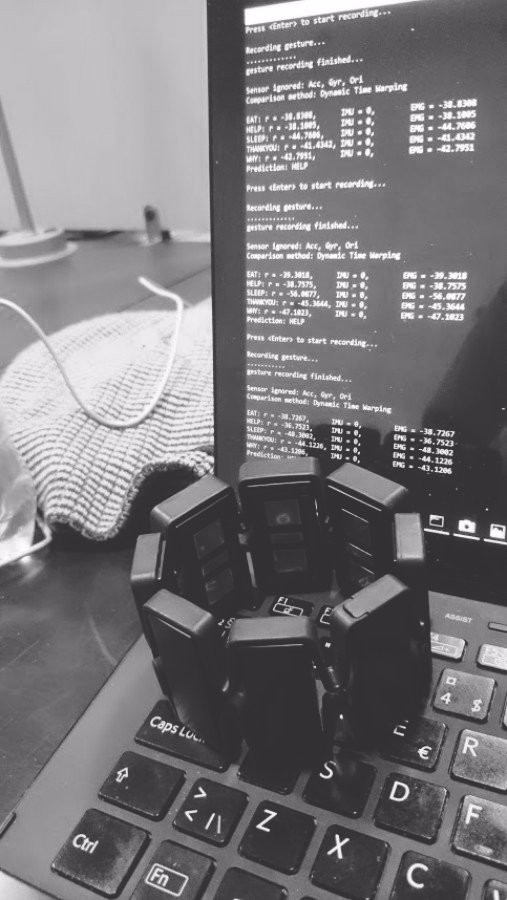
\includegraphics[height=5cm]{content/05-Methodology/images/system_photo.jpg}
        \caption{}
        \label{fig:myo_system_photo}
    \end{subfigure}
    \caption[System illustration]{(\subref{fig:myo_deployment}) A user wearing the Myo armband performing a gesture. (\subref{fig:myo_system_photo}) The Myo armband connected to the implemented system on a Windows computer. }
    \label{fig:system_figure}
\end{figure}

\section{Gesture recording}
The implemented system is not an on-demand gesture recognition solution, but rather an interrupt-based gesture recognition system. To test gestures the user is requested to press enter before the start of the gesture. After the button is pressed, the user have a given time to preform the gesture. The given time is not determined by an actual time variable, but by the numbers of sampling from the sensors given by $n_{s}$, such that
\begin{equation}
\label{eq:data_size_eq}
    n_{s} = f_{s} * t
\end{equation}
where $s$ is a given sensor, $f_{s}$ is the sampling frequency of sensor $s$, and $t$ is the given time. The sampling frequency of the EMG-sensor is 200 hz, and 50 hz for accelerometer, gyroscope and magnetometer, as mentioned in \cref{sec:myoSDK}. The gesture recording stops, when all of the sensors have archived a sampling set of size $n_{s}$.

The recorded gesture is used for comparison with the training set of defined ASL signs. The methods for data comparison is described in detail in \cref{sec:data_comparison}. A diagram of the process from recording a gesture to calculate a similarity rating is illustrated in \cref{fig:gesture_process_diagram}. \Cref{fig:recording_printscreen} shows a print screen of the system while it analyse an input data set.

\begin{figure}[ht]
    \centering
    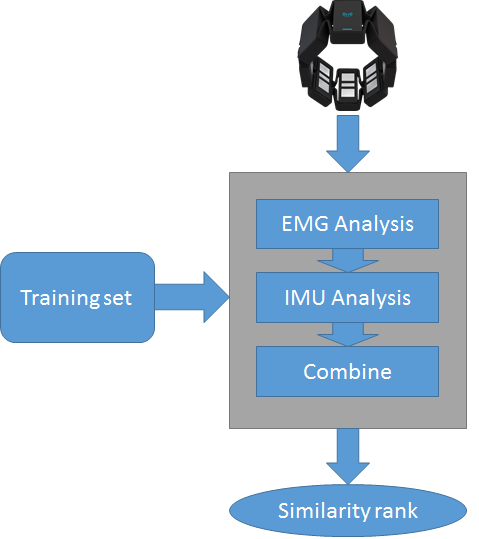
\includegraphics[height=9.5cm]{content/05-Methodology/images/Process_diagram.png}
    \caption[Process Diagram]{A diagram of the progress from recording a gesture to calculate a similarity rank.}
    \label{fig:gesture_process_diagram}
\end{figure}

\begin{figure}[ht]
    \centering
    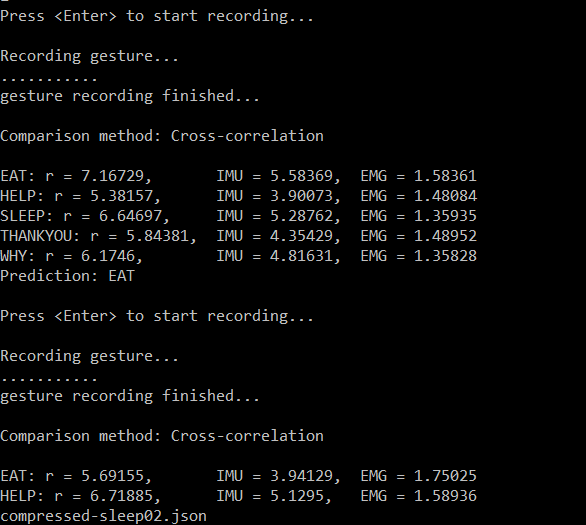
\includegraphics[height=9.5cm]{content/05-Methodology/images/recording.png}
    \caption[Gesture Recording]{A print screen of the system analysing the recorded input.}
    \label{fig:recording_printscreen}
\end{figure}

\section{Training Data}
\label{sec:traning_data}
The method used for gesture recognition uses a comparison method that compare the input with a predefined set of training data, a more detailed view of the comparison method is described in \cref{sec:data_comparison}. This section will cover the training set in detail. Each defined ASL sign have three instances of JSON-files containing the training data for the ASL sign.

\subsection{Data acquisition}
\label{subsec:data_acquisition}
Pewter is an open-source project developed by Ayushman Dash for acquisition, analysis and visualisation of raw data from the Myo Armband \cite{github:pewter}. Pewter is implemented using Node.js, which is a JavaScript runtime environment that is mostly used for developing web applications. The system provide a simple method to record raw data from the Myo armband, and store the recorded data in JSON-format. In addition it provide a visualisation page, where the data is represented in graphs.

\subsection{File Compression}
\label{subsec:file_compress}
Pewter described in \cref{subsec:data_acquisition} provide a simple method for recording gestures, but does not provide any methods to ensure a constant size of the recorded data. The recorded data have to be large enough to cover the gestures, but too large files causes the data analysis to be slow. 

All the raw files recorded from Pewter are recorded with an amount of unnecessary data, a margin to ensure that all the recorded data are within a certain time interval of approximately four seconds. The data for the actual gesture are below a time interval of two seconds. The implemented system provide a method to compress the JSON-files from Pewter to JSON-files with a constant data size given by a set time variable. The size of the data is not determined by the timestamps extractable from the raw JSON-files, but rather calculated using the sample-frequency of the sensors, using the same \cref{eq:data_size_eq} as for gesture recording.
\section{Data Comparison}
\label{sec:data_comparison}
Different comparison methods was used for data comparison. Looking on the graph representation of the data, we can see a visual similarity of the graphs. \Cref{fig:visual_IMU_similarity_example} shows an example of two independent graphs of the orientation x-element data of the same gesture. Similarity of graphs can be determined by method such as Dynamic Time Wrapping and Cross-Correlation, which is described in \cref{subsec:dtw} and \ref{subsec:cross_correlation}. 

\begin{figure}[!ht]
    \centering
    \begin{subfigure}{.5\textwidth}
        \centering
        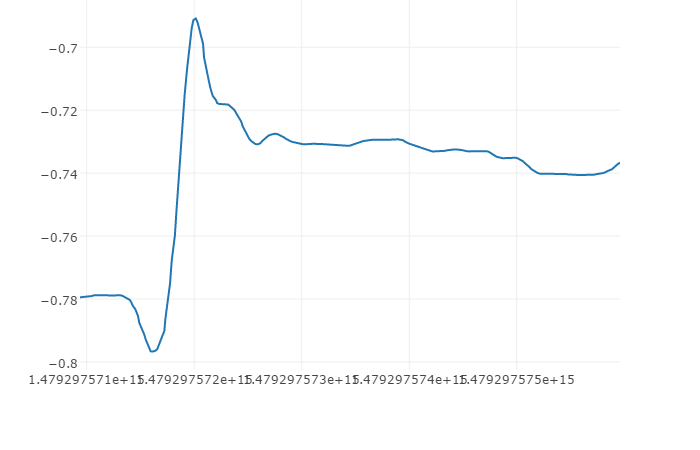
\includegraphics[height=4.5cm]{content/05-Methodology/images/eat-ori-x1.png}
        \caption{}
        \label{fig:eat_ori_x1}
    \end{subfigure}%
    \begin{subfigure}{.5\textwidth}
        \centering
        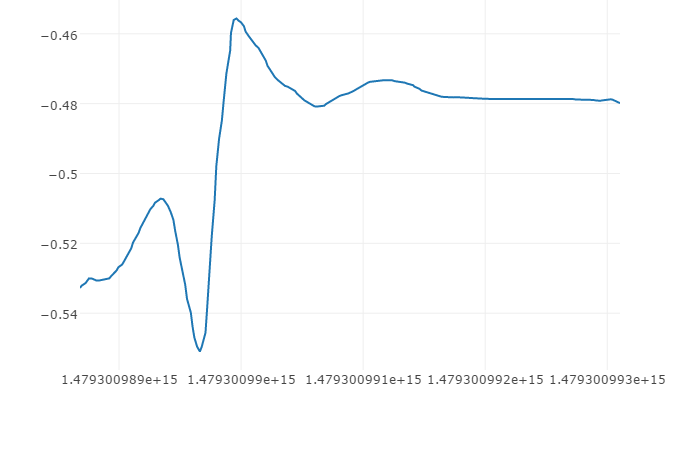
\includegraphics[height=4.5cm]{content/05-Methodology/images/eat-ori-x2.png}
        \caption{}
        \label{fig:eat_ori_x2}
    \end{subfigure}
    \caption[Visual similarity of two IMU-graphs]{The two graphs \subref{fig:eat_ori_x1} and \subref{fig:eat_ori_x2} are two independent graphs of the orientation x-element data of the same gesture. We can see some characteristics that are similar, especially where the graph is increasing and decreasing.}
    \label{fig:visual_IMU_similarity_example}
\end{figure}

Graphs from the EMG data do have similar characteristic as seen in \Cref{fig:visual_EMG_similarity_example}, but the graphs are too noisy to give a good result for comparison methods such as DTW and cross correlation. However, with some data processing we can allow the system to use DTW and cross correlation to analyse the graphs, more details on this is described in \cref{subsec:emg_analysis}.  
\begin{figure}[!ht]
    \centering
    \begin{subfigure}{.5\textwidth}
        \centering
        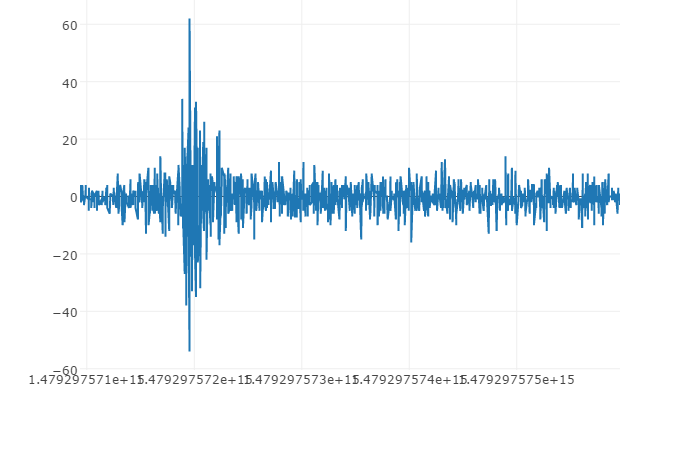
\includegraphics[height=4.5cm]{content/05-Methodology/images/eat-emg8-1.png}
        \caption{}
        \label{fig:eat_emg8_1}
    \end{subfigure}%
    \begin{subfigure}{.5\textwidth}
        \centering
        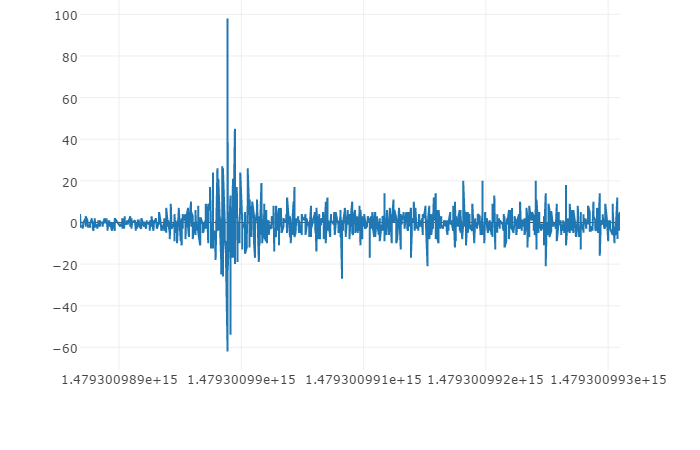
\includegraphics[height=4.5cm]{content/05-Methodology/images/eat-emg8-2.png}
        \caption{}
        \label{fig:eat_emg8_2}
    \end{subfigure}
    \caption[Visual similarity of two EMG-graphs]{The two graphs \subref{fig:eat_emg8_1} and \subref{fig:eat_emg8_2} are two independent graphs of the EMG data from the same pad of the same gesture. We can see similarity of this graphs, but unlike \cref{fig:visual_IMU_similarity_example} there is a lot of noises.}
    \label{fig:visual_EMG_similarity_example}
\end{figure}

\subsection{Dynamic Time Wrapping}
\label{subsec:dtw}
Dynamic time warping (DTW) is a well-known technique to find an optimal alignment between two given (time-dependent) sequences $x$ and $y$ under certain restrictions \cite{muller2007dynamic}. The goal is to align two sequence of graph by warping the time axis iteratively until an optimal match between the two graph is found.

DTW algorithm work with that it tries to fill a cost matrix. Each element of the cost matrix $C$ is the distance of the corresponding elements of the two sequences. Calculating C have a complexity of $\mathcal{O}(n^2)$ where $n$ and $m$ is the size of $x$ and $y$. We can define initial values of C as
\begin{align*}
    C_{0,0} &= D(x_{0},y_{0})  \\
    C_{i,0} &= C_{i-1,0} + D(x_{i},y_{0}) \\
    C_{0,j} &= C_{0,j-1} + D(x_{0},y_{j}) \\
\end{align*}
 and use this to calculate C, such that
\begin{align*}
    C_{i,j} &= min(C_{i - 1,j}, C_{i,j - 1}, C_{i - 1,j - 1}) + D(x_{i}, y_{j}) \\
\end{align*}
where $D(x_{i},y_{j})$ is the euclidean distance between the points $x_{i}$ and $y_{j}$, defined as
\begin{equation*}
    D(x_{i},y_{j}) = \sqrt{(x_{i}-y_{j})^2}
\end{equation*}
The function to calculate Dynamic Time Warping Distance returns $C_{n,m}$, in other word the last element of the matrix.

The similarity of an input to a gesture is calculated by
\begin{equation*}
    d_{g} = \sum_{s}\sum_{i}(\mean{d}_{g,i,s})
\end{equation*}
where $d_{g}$ is the distance value to gesture $g$, and $\mean{d}_{g,i,s}$ is the average distance value given from sensor $s$ of the input to an instance $i$ of the training data sets of gesture $g$. Normalized value $\hat{d}_{g}$ is given by
\begin{equation*}
    \hat{d}_{g} = 1 - \frac{d_{g}}{d_{max}}
\end{equation*}


\subsection{Cross Correlation}
\label{subsec:cross_correlation}
Cross Correlation is a method to estimate the degree of similarity of two series. Cross correlation works on any number of dimension, but for the purpose of this project, we only need to take a look at the one-dimensional cross correlation. Let $x$ and $y$ be two series, then we can define the one-dimensional normalized cross correlation $r$ at delay $d$ as	

\begin{equation}
\label{eq:cross_correlation}
    r(d) = \frac{\sum\limits_{i=0}\limits^{n} [(x(i) - \mean{x}) * (y(i-d) - \mean{y})]}{\sqrt{\sum\limits_{i=0}\limits^{n} (x(i) - \mean{x})^{2}} * \sqrt{\sum\limits_{i=0}\limits^{n} (y(i-d) - \mean{y})^{2}}},
\end{equation}

where $n$ is the number of point and $\mean{x}$ and $\mean{y}$ are the means of the corresponding series \cite{cross_correlation_theory}. The cross correlation have a range of -1 to 1. The value gives information about the series rises and falls relative to each other, where 0 indicating no correlation, $r > 0$ indicating positive correlation and $r < 0$ indicating negative correlation. If both rise at an identical rate, then we have $r = 1$, and opposite $r = -1$ if they fall at an identical rate. 

Given by the formula \ref{eq:cross_correlation} we get an issue when the index is less than 0 or when the index is greater than or equal to the number of points. The most common approach is to ignor this points and let $y(k) = 0$ if $k < 0$ or $k \geq n$ \cite{cross_correlation_code}.

The complexity of the cross correlation algorithm used in the system is $\mathcal{O}(n*k)$, where $n$ is the size of $x$ and $y$, and $k$ is the maximum delay.

The comparison method using cross correlation for an input to a gesture is based on this given equation
\begin{equation*}
    r_{g} = \sum_{s}\sum_{i}\mean{r}_{g,i,s} 
\end{equation*}
where $r_{g}$ is the correlation value to gesture $g$, and $\mean{r}_{g,i,s}$ is the average cross-correlation value given from sensor $s$ of the input to an instance $i$ of the training data sets of gesture $g$. Perfect correlation is given by
\begin{equation*}
    r_{max} = a*c
\end{equation*}
where $a$ is the number of training instance for each defined ASL sign and $c$ is the number of used sensors in the analysis.

\subsection{EMG Analysis}
\label{subsec:emg_analysis}
While DTW and cross-correlation works fine for the raw data from the IMU-sensors, EMG is a bit harder to analyse. \Cref{fig:visual_EMG_similarity_example} shows a side by side comparison of the EMG data from the same pod of the same gesture. DTW and cross-correlation dose not give applicable results from this kind of nosy graphs, and we have to preprocess the raw EMG-date before we can use DTW or cross-correlation to analyse similarities.

However, Looking at different graph representations of raw EMG-data we can see some visual similarities of the intensity of high-value outputs. By dividing the data into intervals of size $n_{interval}$, we can find those intense high-value outputs. Let $E_{old}$ be the raw data set of EMG-data and $E$ be a new data set given by 

\begin{equation*}
    E[i] = \sum\limits_{j=k}\limits^{k + n_{interval}}\frac{E_{old}[j]^2}{maxSq(E_{old})} 
\end{equation*}

where $k = i*n_{interval}$ and $i$ is the index of the interval. $maxSq(E_{old})$ is the highest squared value of $E_{old}$. The new data set $E$ gives some information of the occurrence of the high-valued outputs. We can use DTW and cross-correlation on the new data set.
\chapter{Results}
\label{chap:results}
This chapter will cover preliminary for the test and the test result collected from the test. The results will be further discussed in \cref{chap:discussion}.

\section{Preliminary}
The system is only intended to test the potential for the Myo armband, and therefore will have only 5 defined ASL signs, that are described in \cref{table:ASL_signs}. The ASL signs are randomly selected from the ASL dictionary \cite{ASL_dict}. 

\begin{table}[ht!]
\centering
    \begin{tabular}{ | l | p{4cm} | p{7cm}|}
        \hline
        \textbf{ASL name} & \textbf{Location} & \textbf{Movement disciption} \\ \Xhline{4\arrayrulewidth}
        
        \textbf{Eat} & Mouth & Upward toward the mouth with a beak-formed hand. Small back and forward motion near the mouth. \\ \hline
        
        \textbf{Help} & Thorax & Hammer-like motion over the other hand at thorax level height.\\ \hline
        
        \textbf{Sleep} & Nose & Open hand to nose level, then lower the arm to right bellow the chin while making a fist on the way.\\ \hline
        
        \textbf{Thank you} & Mouth & Open hand toward mouth, then half down again.\\ \hline
        
        \textbf{Why} & Upper head & Open hand toward uper head, then hand away from the head while making a fist with the thumb and pinky finger pointing upward.\\ \hline
    \end{tabular}
    \caption[Defines ASL signs]{List of ASL signs used for the testing of the system.}
    \label{table:ASL_signs}
\end{table}

All the gestures have three instances of training data, which seemed sufficient for a good result. The training instances is recorded on different time, to make sure it represent a good variety of data of the same gesture. All the results shown in \cref{sec:test_results} are from tests done on the same user. The test data is pre-recorded so that all the tests can work on the same data set. For each gesture we have ten instances of test data set.

All the training and test instances is done with some initial setups, that is
\begin{itemize}
    \item Myo armband placement on arm, and
    \item start position of arm
\end{itemize}
The system does not provide any pre-processing analysis to calculate the position of the Myo armband on the arm or the start position of the gesture. EMG from different positions on the arm have different values, and the system is dependent on that the data from the pads match with the placement of the pad when the training instances was recorded.

The tests tries to compare the utilization of IMU-sensor and EMG-sensors, by letting the recognition system exclude data from given a sensor. This report will not cover exclusion of each individual sensor, but treat the IMU-sensors as one instance. The results show both the results for test with DTW and Cross correlation.  

\section{Raw Results}
This section will provide some of the raw result for the tests. 

\begin{table}[H]
\centering
    \begin{tabular}{  l  p{3cm}  p{3cm} p{3cm}}
        \multicolumn{3}{l}{Test file: test-sleep02.json} \\
        \multicolumn{3}{l}{Comparison method: Dynamic Time Warping} \\[0.3cm]
        \hline
        \textbf{Gesture} & \textbf{r} & \textbf{IMU} & \textbf{EMG} \\ \Xhline{4\arrayrulewidth}
        
        \textbf{Eat} & 2.05578 &  1.79945 & 0.256333 \\ 
        
        \textbf{Help}  & 0.153523 &  0 & 0.153523 \\ 
        
        \textbf{Sleep}  & 2.04685 &  2.02115 & 0.0257067 \\ 
        
        \textbf{Thank you} & 0.95783 &  0.892639 & 0.0651904 \\ 
        
        \textbf{Why} & 1.82603 &  1.82603 & 0 \\ 
        \hline
        
        \multicolumn{3}{l}{Gesture: SLEEP} \\
        \multicolumn{3}{l}{Result: EAT}\\
    \end{tabular}
    \caption[Raw Result of DTW]{Raw result output using DTW}
    \label{table:raw_result_test-sleep02_DTW}
\end{table}

\begin{table}[H]
\centering
    \begin{tabular}{  l  p{3cm}  p{3cm} p{3cm}}
        \multicolumn{3}{l}{Test file: test-sleep02.json} \\
        \multicolumn{3}{l}{Comparison method: Cross-correlation} \\[0.3cm]
        \hline
        \textbf{Gesture} & \textbf{r} & \textbf{IMU} & \textbf{EMG} \\ \Xhline{4\arrayrulewidth}
        
        \textbf{Eat} & 8.55614 &  6.95654 & 1.5996 \\ 
        
        \textbf{Help}  & 6.06123 &  4.41452 & 1.6467 \\ 
        
        \textbf{Sleep}  & 9.12446 &  7.61892 & 1.50554 \\ 
        
        \textbf{Thank you} & 7.37875 &  5.90616 & 1.4726 \\ 
        
        \textbf{Why} & 8.29722 & 6.79873 & 1.49849 \\ 
        \hline
        
        \multicolumn{3}{l}{Gesture: SLEEP} \\
        \multicolumn{3}{l}{Result: SLEEP}\\
    \end{tabular}
    \caption[Raw Result of Cross correlation]{Raw result output using cross correlation}
    \label{table:raw_result_test-sleep02_cross_correlation}
\end{table}

\section{Test Results}
\label{sec:test_results}

% DTW
\begin{table}[ht!]
\centering
    \begin{tabular}{ | l | p{4cm} | p{4cm}|}
        \hline
        \textbf{Gesture} & \textbf{Correct Recognized Gestures} & \textbf{Number Of Tests} \\ \Xhline{4\arrayrulewidth}
        
        \textbf{Eat} & 9 &  10 \\ \hline
        
        \textbf{Help}  & 10 &  10 \\ \hline
        
        \textbf{Sleep}  & 2 &  10 \\ \hline
        
        \textbf{Thank you}  & 10 &  10 \\ \hline
        
        \textbf{Why}  & 10 &  10 \\ \hline
    \end{tabular}
    \caption[DTW test]{DTW}
    \label{table:DTW_test}
\end{table}

%DTW without EMG
\begin{table}[ht!]
\centering
    \begin{tabular}{ | l | p{4cm} | p{4cm}|}
        \hline
        \textbf{Gesture} & \textbf{Correct Recognized Gestures} & \textbf{Number Of Tests} \\ \Xhline{4\arrayrulewidth}
        
        \textbf{Eat} & 9 &  10 \\ \hline
        
        \textbf{Help}  & 10 &  10 \\ \hline
        
        \textbf{Sleep}  & 6 &  10 \\ \hline
        
        \textbf{Thank you}  & 10 &  10 \\ \hline
        
        \textbf{Why}  & 10 &  10 \\ \hline
    \end{tabular}
    \caption[DTW without EMG test]{DTW without EMG}
    \label{table:DTW_without_EMG_test}
\end{table}

%DTW without IMU
\begin{table}[ht!]
\centering
    \begin{tabular}{ | l | p{4cm} | p{4cm}|}
        \hline
        \textbf{Gesture} & \textbf{Correct Recognized Gestures} & \textbf{Number Of Tests} \\ \Xhline{4\arrayrulewidth}
        
        \textbf{Eat} & 10 &  10 \\ \hline
        
        \textbf{Help}  & 3 &  10 \\ \hline
        
        \textbf{Sleep}  & 3 &  10 \\ \hline
        
        \textbf{Thank you}  & 1 &  10 \\ \hline
        
        \textbf{Why}  & 0 &  10 \\ \hline
    \end{tabular}
    \caption[DTW without IMU]{DTW without IMU}
    \label{table:DTW_without_IMU_test}
\end{table}

% Cross-correlation
\begin{table}[ht!]
\centering
    \begin{tabular}{ | l | p{4cm} | p{4cm}|}
        \hline
        \textbf{Gesture} & \textbf{Correct Recognized Gestures} & \textbf{Number Of Tests} \\ \Xhline{4\arrayrulewidth}
        
        \textbf{Eat} & 8 &  10 \\ \hline
        
        \textbf{Help}  & 10 &  10 \\ \hline
        
        \textbf{Sleep}  & 9 &  10 \\ \hline
        
        \textbf{Thank you}  & 10 &  10 \\ \hline
        
        \textbf{Why}  & 10 &  10 \\ \hline
    \end{tabular}
    \caption[Cross-correlation test]{Cross-correlation}
    \label{table:cross_correlation_test}
\end{table}

% Cross-correlation without EMG
\begin{table}[ht!]
\centering
    \begin{tabular}{ | l | p{4cm} | p{4cm}|}
        \hline
        \textbf{Gesture} & \textbf{Correct Recognized Gestures} & \textbf{Number Of Tests} \\ \Xhline{4\arrayrulewidth}
        
        \textbf{Eat} & 8 &  10 \\ \hline
        
        \textbf{Help}  & 10 &  10 \\ \hline
        
        \textbf{Sleep}  & 8 &  10 \\ \hline
        
        \textbf{Thank you}  & 10 &  10 \\ \hline
        
        \textbf{Why}  & 10 &  10 \\ \hline
    \end{tabular}
    \caption[Cross-correlation without EMG test]{Cross-correlation without EMG}
    \label{table:cross_correlation_without_EMG_test}
\end{table}

% Cross-correlation without IMU
\begin{table}[ht!]
\centering
    \begin{tabular}{ | l | p{4cm} | p{4cm}|}
        \hline
        \textbf{Gesture} & \textbf{Correct Recognized Gestures} & \textbf{Number Of Tests} \\ \Xhline{4\arrayrulewidth}
        
        \textbf{Eat} & 7 &  10 \\ \hline
        
        \textbf{Help}  & 7 &  10 \\ \hline
        
        \textbf{Sleep}  & 3 &  10 \\ \hline
        
        \textbf{Thank you}  & 1 &  10 \\ \hline
        
        \textbf{Why}  & 2 &  10 \\ \hline
    \end{tabular}
    \caption[Cross-correlation without IMU]{Cross-correlation without IMU}
    \label{table:cross_correlation_without_IMU_test}
\end{table}

% Cross-correlation without IMU
\begin{table}[ht!]
\centering
    \begin{tabular}{ | l | p{4cm} | p{4cm}|}
        \hline
        \textbf{Gesture} & \textbf{Correct Recognized Gestures} & \textbf{Number Of Tests} \\ \Xhline{4\arrayrulewidth}
        
        \textbf{Eat} & 1 &  10 \\ \hline
        
        \textbf{Help}  & 9 &  10 \\ \hline
        
        \textbf{Sleep}  & 2 &  10 \\ \hline
        
        \textbf{Thank you}  & 4 &  10 \\ \hline
        
        \textbf{Why}  & 1 &  10 \\ \hline
    \end{tabular}
    \caption[Cross-correlation on raw EMU]{Cross-correlation on raw EMU-data}
    \label{table:cross_correlation_raw_EMG_test}
\end{table}
\chapter{Discussion}
\label{chap:discussion}

\section{Future Work}
\chapter{Conclusion}
\label{chap:conclusion}


% Bibliography - edit references.bib and use the \cite command in text
\renewcommand{\bibname}{References}
\bibliographystyle{plain}
\bibliography{references}
\clearpage

\pagenumbering{arabic}% resets `page` counter to 1
\renewcommand*{\thepage}{A-\arabic{page}}

\phantomsection
\addcontentsline{toc}{chapter}{Appendix}
\clearpage
\vspace*{\fill}
{\centering\huge\bfseries Appendix \par}
\vspace*{\fill}
\thispagestyle{empty}

\clearpage

\printglossary[type=abbreviation, title=Abbreviations, nonumberlist, style=custom_super] % print the glossary

\end{document}